
\begin{frame}[fragile,t]{Histórico da Linguagem Ruby}
  \begin{itemize}
    \item Inventada por Yukihiro "Matz" Matsumoto
    \item Verão 1.0 liberada em 1996(Japão)
    \item Popularizado no início de 2005 pelo Rails
  \end{itemize}   
  \begin{figure}[hbt]
    
\includegraphics[scale=.5]{imagens/matz.png}
  \end{figure}
\end{frame}

\begin{frame}[fragile,t]{Visão Geral}
  \begin{itemize}
    \item Dinâmica
    \item Orientada a Objetos
    \item Elegante, expressiva e declarativa
    \item Influenciada pelo Perl, Smalltalk, Eiffel e Lisp
    \item Projeta para tornar o programador "Feliz"
  \end{itemize}   
\end{frame}

\begin{frame}[fragile,t]{..Java..}
  \begin{lstlisting}[style=JavaInputStyle]
    public class Print3Times {
      public static void main(String[] args) {
        for(int i = 0; i < 3; i++) {
          System.out.println("Hello World!")
        }
      }
    }
  \end{lstlisting}
\end{frame}

\begin{frame}[fragile,t]{..Ruby..}
  \begin{lstlisting}[style=RubyInputStyle]
    3.times {puts "Hello World!"}
  \end{lstlisting}
\end{frame}

\begin{frame}[fragile,t]{Básico do Ruby}
  \begin{itemize}
    \item Indentação de 2 espaços para cada nível aninhado (recomendado)
    \item \# é utilizado para comentários
    \begin{itemize}
    	\item use com moderacao, o código deve ser auto documentado
    \end{itemize}
    \item Scripts utilizam a extensão \verb!.rb!
    
	\lstinputlisting[style=RubyInputStyle, caption=codigos/ruby/01-ruby-introducao/introducao.rb]{codigos/ruby/01-ruby-introducao/introducao.rb}
  \end{itemize}   
\end{frame}

\begin{frame}[fragile,t]{Impressão na Tela}
  \begin{itemize}
    \item \verb!puts! é método padrão para impressão em tela 
    \begin{itemize}
    	\item insere uma quebra de linha após a impressão
    	\item similar ao \verb!System.out.println! do Java
    \end{itemize}
  \end{itemize}   
\end{frame}

\begin{frame}[allowframebreaks,fragile,t]{Executando um Script Ruby}
  \begin{figure}[hbt]
    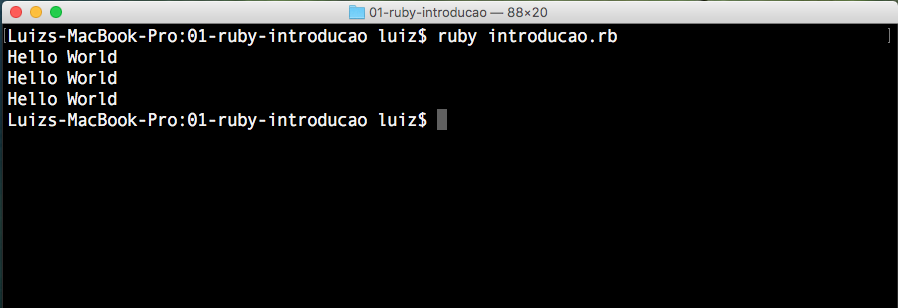
\includegraphics[scale=.25]{imagens/ruby-interpretador.png}
  \end{figure}
\end{frame}

\begin{frame}[fragile,t]{Convenção de Nomes}
  \begin{itemize}
    \item Variáveis e Métodos
    \begin{itemize}
    	\item em minúsculas e \verb!separada_por_sublinhado! (tenha mais de uma palavra)
    	\item métodos ainda permitem no final os caracteres \verb|?!|
    \end{itemize}
    \item Constantes
    \begin{itemize}
    	\item tanto \verb!TODAS_AS_LETRAS_EM_MAIUSCULAS! ou no formato \verb!CamelCase!
    \end{itemize}
    \item Classes(e módulos)
    \begin{itemize}
    	\item formato \verb!CamelCase! 
    \end{itemize}
  \end{itemize}
\end{frame}

\begin{frame}[fragile,t]{Remoção do Ponto-e-Vírgula}
  \begin{itemize}
    \item Não coloque o ponto-e-vírgula no final da linha
    \item Pode ser utilizado para colocar várias declarações em uma linha
    \begin{itemize}
      \item altamente desencorajado
    \end{itemize}
    \begin{lstlisting}[style=RubyInputStyle]
      a = 3	
      a = 3; b = 5 
    \end{lstlisting}
  \end{itemize}
\end{frame}

\begin{frame}[fragile,t]{Interactive Ruby (IRB)}
  \begin{itemize}
    \item Console interativa para interpretação de comandos Ruby
    \item Instalado com o interpretador Ruby
    \item Permite a execução de comandos rapidamente
  \end{itemize}
  \begin{figure}[hbt]
    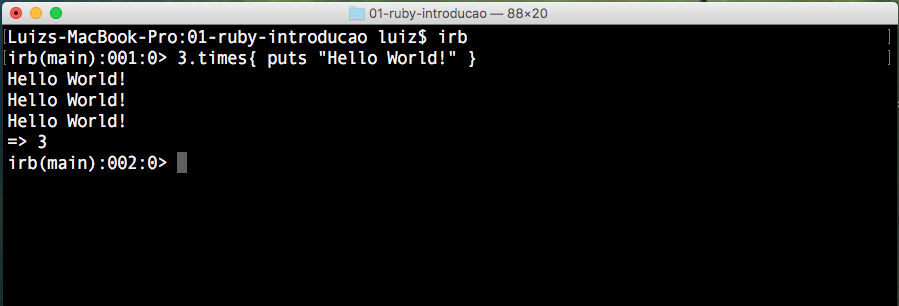
\includegraphics[scale=.25]{imagens/ruby-irb.png}
  \end{figure}
\end{frame}


